\section{Tarefas (Issues)}\label{tarefas-issues}

Veja as tarefas disponíveis em:
\url{https://github.com/ifce-gp-20151/saa/issues}

\begin{figure}[H]
    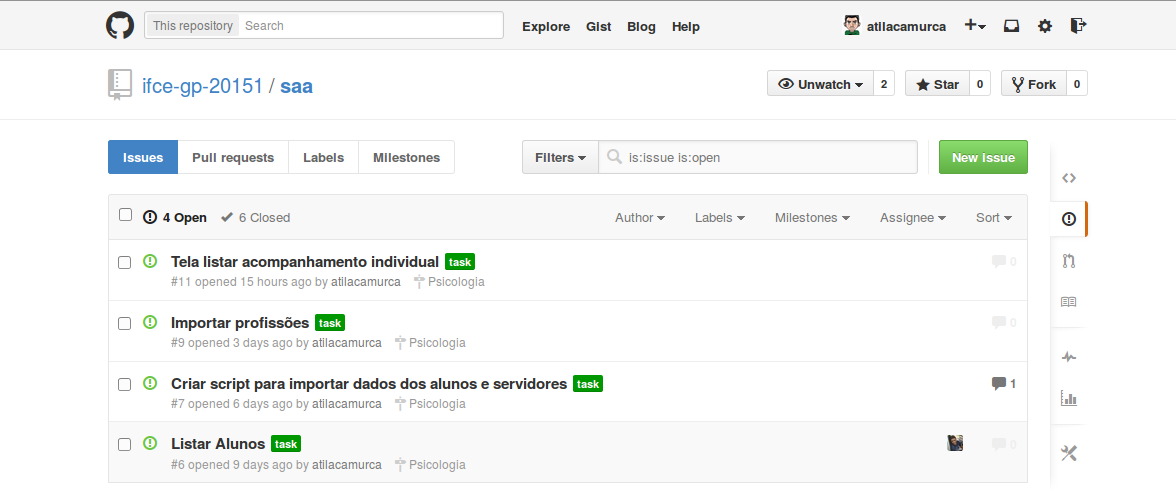
\includegraphics[scale=0.4]{img/issues.png}
    \caption{Página de issues}
\end{figure}

Clique na tarefa que deseja resolver e indique que você irá resolver.

\begin{figure}[H]
    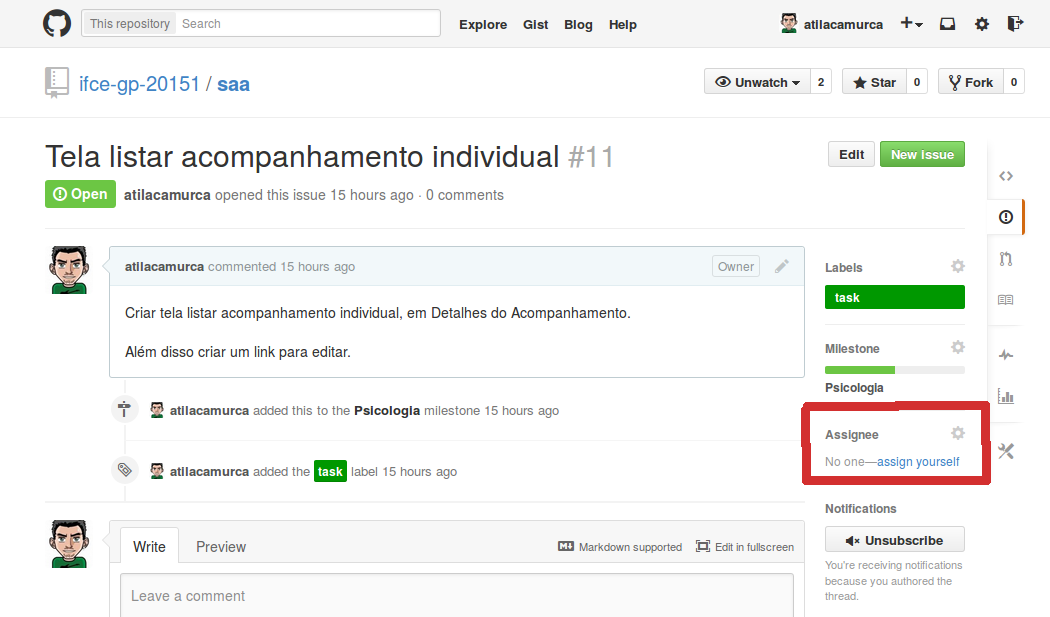
\includegraphics[scale=0.4]{img/resolver-issue.png}
    \caption{Resolver issue}
\end{figure}

Verifique o número da issue. Ela vai ser o nome do seu \emph{branch}
local.

\begin{figure}[H]
    
\includegraphics[scale=0.5]{img/numero-issue.png}
    \caption{Número da issue}
\end{figure}

\section{Branch no repositório
local}\label{branch-no-reposituxf3rio-local}

Entre em seu repositório local pelo terminal e crie o branch de acordo
com o número da issue.

\begin{verbatim}
git checkout master
git fetch origin
git merge origin/master
git checkout -b issue-11
\end{verbatim}

Começe a trabalhar normalmente.

Verifique a pasta \texttt{./docs/manual/workflow-zend}.

\section{Finalizar tarefa}\label{finalizar-tarefa}

Ao finalizar a tarefa você deve fazer \emph{commit} de suas alterações.
Para facilitar use o \texttt{gitg}. Para utilizar basta executar no seu
repositório local \texttt{gitg}.

\begin{figure}[H]
    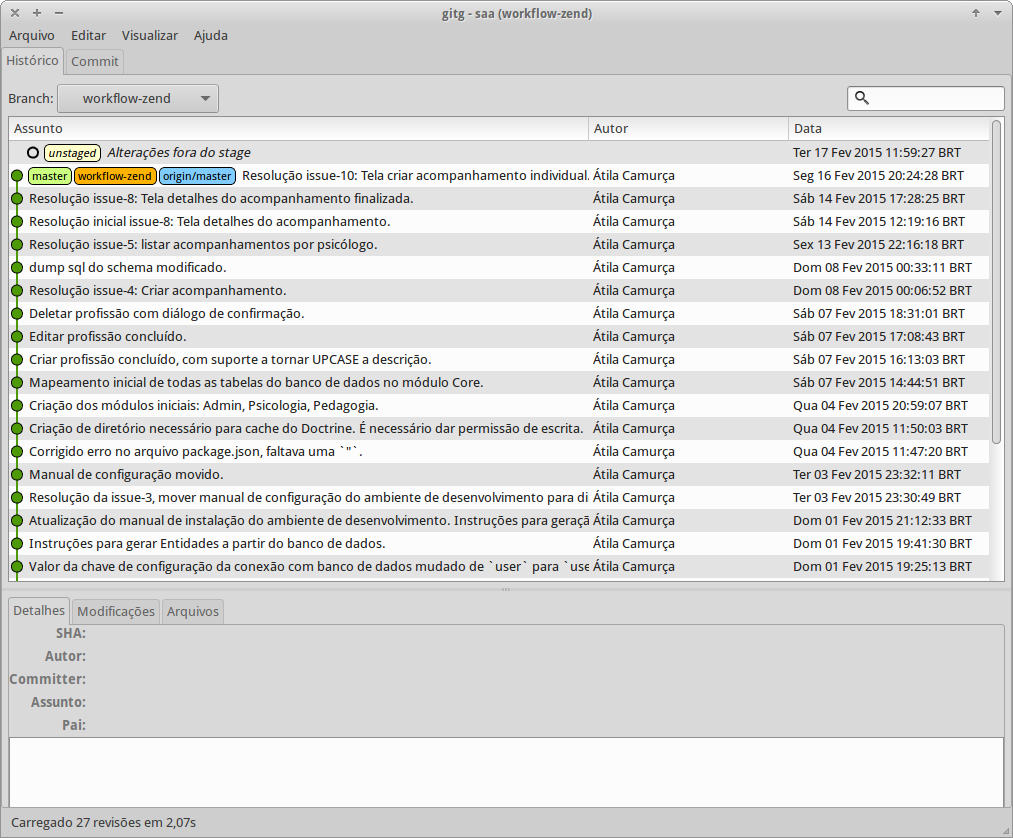
\includegraphics[scale=0.4]{img/gitg.png}
    \caption{gitg}
\end{figure}

Verifique se o \emph{branch} está correto:

\begin{figure}[H]
    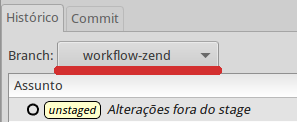
\includegraphics[scale=1.0]{img/gitg-branch.png}
    \caption{Branch}
\end{figure}

\textbf{Obs.:} no exemplo está com outro nome, mas no caso deveria ter o
valor \textbf{issue-11}.

\subsection{Commit das alterações}\label{commit-das-alterauxe7uxf5es}

Para fazer o \emph{commit} clique na aba Commit. Coloque os arquivos
necessários de \emph{Unstaged} para \emph{Staged}. Por fim escreva a
mensagem de \emph{commit}, e clique no botão \textbf{Commit}:

\begin{figure}[H]
    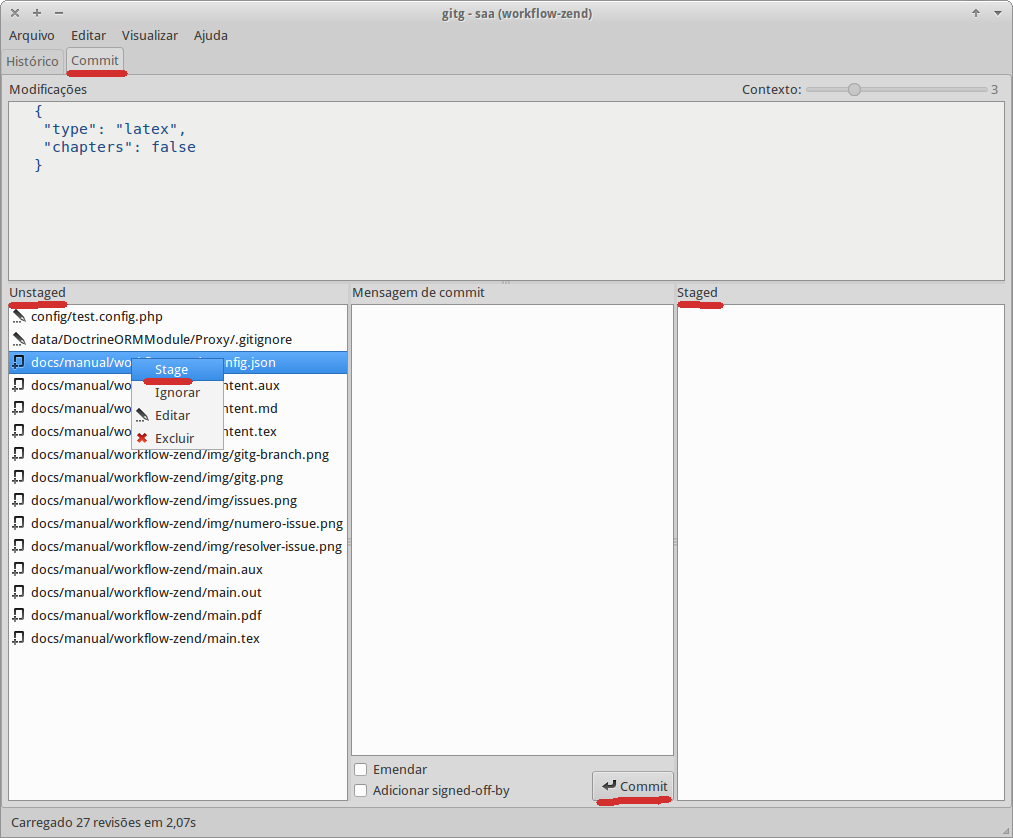
\includegraphics[scale=0.4]{img/gitg-commit.png}
    \caption{Commit}
\end{figure}

Feche o \texttt{gitg}.

\section{Atualizar com o código
Remoto}\label{atualizar-com-o-cuxf3digo-remoto}

Antes de subir as alterações é necessário atualizar a base com o
repositório remoto. Para isso faça:

\begin{verbatim}
git checkout master
git fetch origin
git merge origin/master
\end{verbatim}

Logo depois faça o \emph{merge} com o seu \emph{branch}:

\begin{verbatim}
git checkout master
git merge issue-11
\end{verbatim}

A saída será algo como:

\begin{verbatim}
Updating f42c576..3a0874c
Fast-forward
 index.html | 2 ++
 1 file changed, 2 insertions(+)
\end{verbatim}

Verifique se \texttt{Fast-foward} aparece na mensagem. Isso quer dizer:
``Ok, tudo certo para subir o código!''.

\begin{verbatim}
git push -u origin master
\end{verbatim}

\subsection{Conflitos!}\label{conflitos}

Podem acontecer conflitos ao fazer o \emph{merge}, ou seja, seu código
possui linhas de código modificadas no mesmo local que as do repositório
remoto. Quando isso acontecer ao fazer o \emph{merge} a saída será algo
como:

\begin{verbatim}
Auto-merging index.html
CONFLICT (content): Merge conflict in index.html
Automatic merge failed; fix conflicts and then commit the result.
\end{verbatim}

A frase final indica:

\begin{quote}
Merge automático falhou; resolva os conflitos e então faça commit do
resultado.
\end{quote}

Para resolver os conflitos use o \texttt{meld}. Instalação:

\begin{verbatim}
sudo apt-get install meld
\end{verbatim}

Em seguida dento do seu repositório local execute:

\begin{verbatim}
git mergetool
\end{verbatim}

Uma mensagem semelhante a essa irá aparecer, apenas dê \texttt{Enter}.

\begin{verbatim}
This message is displayed because 'merge.tool' is not configured.
See 'git mergetool --tool-help' or 'git help config' for more details.
'git mergetool' will now attempt to use one of the following tools:
opendiff meld tortoisemerge bc3 codecompare vimdiff emerge
Merging:
index.html

Normal merge conflict for 'index.html':
  {local}: modified file
  {remote}: modified file
Hit return to start merge resolution tool (meld):
\end{verbatim}

\begin{figure}[H]
    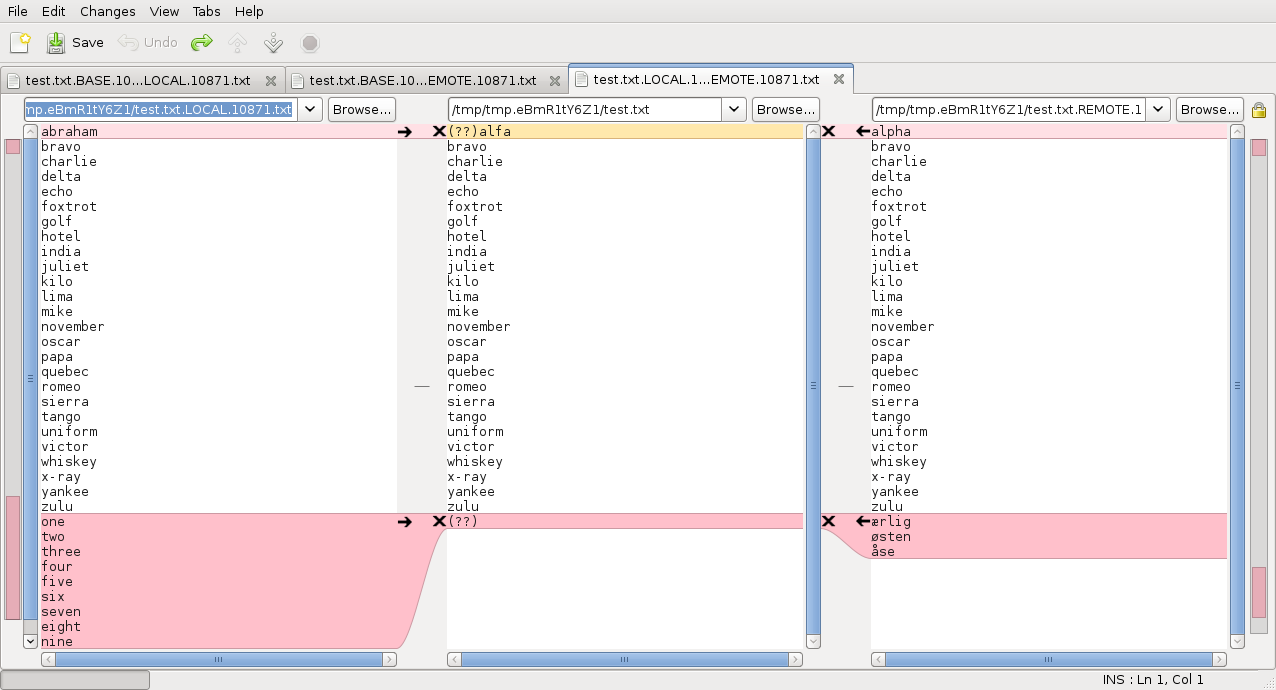
\includegraphics[scale=0.35]{img/meld3.png}
    \caption{Meld}
\end{figure}

Esse é o chamado \emph{Three way git merging}, ou merge de três vias. O
arquivo a esquerda é seu arquivo local, o do meio é o arquivo que é
ancestral, e o da direita o arquivo remoto.

Coloque todas as alterações para o arquivo do meio, clicando na
\texttt{seta}. Clique no \texttt{X} para apagar. Segure \texttt{Ctrl}
para colocar o código abaixo ou acima do indicado, assim é possível
juntar algo do seu \emph{branch} com o do \emph{branch} remoto.

Caso tenha acontecido conflitos em mais de um arquivo, ao fechar o
\texttt{meld} basta continuar dando \texttt{Enter}.
